\begin{name}
{\tenchude}{\tendethi}{LỚP TOÁN THẦY PHÁT}{\thoigian}
\end{name}
\Opensolutionfile{ans}[ans/ansBTTeX1]
\begin{ex}%[2D3Y1-1]%
Họ nguyên hàm của hàm số $f(x)=\dfrac{1}{\sqrt{x^{2}+a}}$ bằng
\choice
{$\ln \left|x-\sqrt{x^{2}+a}\right|+C$}
{\True$\ln \left|x+\sqrt{x^{2}+a}\right|+C$}
{$\ln \left|\sqrt{x^{2}+a}\right|+C$}
{$\ln \left|\sqrt{x^{2}+a}-2 x\right|+C$}
\loigiai{
Công thức $\displaystyle\int \dfrac{1}{\sqrt{x^{2}+a}}\mathrm{\,d}x=\ln \left|x+\sqrt{x^{2}+a}\right|+C$.
}
\end{ex}

\begin{ex}%[2D3Y1-1]%
Hàm số nào sau đây là một nguyên hàm của hàm số $f(x)=\mathrm{e}^{2x}$?
\choice
{\True $F(x)=\dfrac{1}{2}\mathrm{e}^{2x}+2020$}
{$F(x)=2\mathrm{e}^{2x}+1$}
{$F(x)=\dfrac{1}{2}\mathrm{e}^{2x}+x$}
{$F(x)=\mathrm{e}^{2x}+2021$}
\loigiai
{
Ta có $\displaystyle\int f(x) \mathrm{\,d}x=\displaystyle\int \mathrm{e}^{2x} \mathrm{\,d}x=\dfrac{1}{2}\mathrm{e}^{2x}+C$.\\
Khi đó $F(x)=\dfrac{1}{2}\mathrm{e}^{2x}+2020$ là một nguyên hàm của hàm số $f(x)=\mathrm{e}^{2x}$.
}
\end{ex}

\begin{ex}%[2D3B1-1]%
Họ nguyên hàm $F(x)=\displaystyle\int\cos^{2}x\mathrm{\,d}x$ là
\choice
{\True $F(x)=\dfrac{x}{2}+\dfrac{\sin 2x}{4}+C$}
{$F(x)=\dfrac{x}{4}-\dfrac{\cos 2x}{4}+C$}
{$F(x)=\dfrac{x}{3}+\dfrac{\sin 2x}{3}+C$}
{$F(x)=x+\dfrac{\sin 2x}{2}+C$}
\loigiai{
Ta có $F(x)=\displaystyle\int\cos^{2}x\mathrm{\,d}x=\displaystyle\int\dfrac{1+\cos 2x}{2}\mathrm{\,d}x=\dfrac{x}{2}+\dfrac{\sin 2x}{4}+C$.
}
\end{ex}

\begin{ex}%[2D3B1-1]%
Biết $F(x)=(a x^2+b x+c) \sqrt{2x-3}$ là nguyên hàm của hàm số $f(x)=\dfrac{20 x^2-30 x+11}{\sqrt{2x-3}} \cdot$ Giá trị của $a+b+c$ bằng
\choice
{$5$}
{$6$}
{\True $7$}
{$8$}
\loigiai{
Ta có
\begin{eqnarray*}
f(x)&=&F'(x)=(2ax+b)\sqrt{2x-3}+(ax^2+bx+c)\cdot \dfrac{1}{\sqrt{2x-3}}\\
&=& \dfrac{(2ax+b)(2x-3)+ax^2+bx+c}{\sqrt{2x-3}}\\
&=& \dfrac{5ax^2+(3b-6a)x-3b+c}{\sqrt{2x-3}}.
\end{eqnarray*}
Suy ra $\heva{&5a=20\\&3b-6a=-30\\&-3b+c=11}\Rightarrow \heva{&a=4\\&b=-2\\&c=5.}$\\
Giá trị của $a+b+c=7$.
}
\end{ex}

\begin{ex}%[2D3B1-2]%
Họ nguyên hàm của hàm số $f(x)=\dfrac{4^x+1}{2^x}$ là
\choice
{\True $F(x)=\dfrac{2^x}{\ln 2}-\dfrac{1}{2^x\ln2}+C$}
{$F(x)=\dfrac{4^x}{2\ln2}+\dfrac{2^x}{\ln2}+C$}
{$F(x)=\dfrac{2^x}{\ln2}+\dfrac{1}{2^x\ln2}+C$}
{$F(x)=\dfrac{4^x}{\ln2}-\dfrac{2^x}{\ln2}+C$}
\loigiai{
Ta có $\displaystyle\int\dfrac{4^x+1}{2^x}\mathrm{d}x=\displaystyle\int\left(2^x+2^{-x}\right)\mathrm{d}x=\dfrac{2^x}{\ln2}-\dfrac{1}{2^x\ln2}+C$.
}
\end{ex}

\begin{ex}%[2D3B1-3]%
Họ nguyên hàm $F(x)=\displaystyle\int x\mathrm{e}^{2x}\mathrm{d}x$ là
\choice
{$F(x)=(2x-1)\mathrm{e}^{2x}+C$}
{$F(x)=(x-2)\mathrm{e}^{2x}+C$}
{$F(x)=\dfrac{1}{4}(2x+1)\mathrm{e}^{2x}+C$}
{\True $F(x)=\dfrac{1}{2}\left(x-\dfrac{1}{2}\right)\mathrm{e}^{2x}+C$}
\loigiai{
Đặt $\heva{&u=x\\&\mathrm{d}v=\mathrm{e}^{2x}\mathrm{d}x}\Rightarrow\heva{&\mathrm{d}u=\mathrm{d}x\\&v=\dfrac{1}{2}\mathrm{e}^{2x}.}$\\
Khi đó $F(x)=\displaystyle\int x\mathrm{e}^{2x}\mathrm{d}x=\dfrac{1}{2}x\mathrm{e}^{2x}-\displaystyle\int\left(\dfrac{1}{2}\mathrm{e}^{2x}\right)\mathrm{d}x=\dfrac{x\mathrm{e}^{2x}}{2}-\dfrac{\mathrm{e}^{2x}}{4}+C=\dfrac{1}{2}\left(x-\dfrac{1}{2}\right)\mathrm{e}^{2x}+C$.
}
\end{ex}

\begin{ex}%[Câu 17]%[2D3Y2-1]%
Tính tích phân $\displaystyle \displaystyle I=\int\limits_{-1}^1(4x^3-3)\mathrm{\,d}x$.
\choice
{$I=6$}
{\True $I=-6$}
{$I=4$}
{$I=-4$}
\loigiai{
Ta có $\displaystyle \displaystyle I=\int\limits_{-1}^1(4x^3-3)\mathrm{\,d}x=\left. (x^4-3x)\right|_{-1}^1=-6$.}
\end{ex}

\begin{ex}%[2D3Y2-1]%
Giá trị của tích phân $\displaystyle\int\limits_{0}^{\mathrm{e}^{2020}-1} \dfrac{\mathrm{\,d}x}{x+1}$ bằng
\choice
{\True$2020$}
{$2019$}
{$2021$}
{$0$}
\loigiai{
Ta có $\displaystyle\int\limits_{0}^{\mathrm{e}^{2020}-1} \dfrac{\mathrm{\,d}x}{x+1}=\ln(x+1)\bigg|_0^{\mathrm{e}^{2020}-1} =2020$.
}
\end{ex}

\begin{ex}%[Dự án Tex TDM - NHTP - Lê Quân]%[2D3B2-1]%
Biết $\displaystyle\int\limits_{0}^{1}\left[2f(x)+3g(x)\right]\mathrm{\, d}x=12$ và $\displaystyle\int\limits_{0}^{1}\left[4f(x)-g(x)\right]\mathrm{\, d}x=5$. Giá trị của tích phân $\displaystyle\int\limits_{0}^{1}\left[2019f(x)-2020 g(x)\right]\mathrm{\, d}x$ bằng
\choice
{$-\dfrac{201921}{14}$}
{\True $-\dfrac{22247}{14}$}
{$-\dfrac{52247}{28}$}
{$\dfrac{31543}{14}$}
\loigiai{
Đặt $\heva{&\displaystyle\int\limits_{0}^{1}f(x)\mathrm{\, d}x=a    \\&\displaystyle\int\limits_{0}^{1}g(x)\mathrm{\, d}x=b}\Rightarrow \heva{&2a+3b=12 \\&4a-b=5}\Leftrightarrow \heva{&a=\dfrac{27}{14}   \\&b=\dfrac{19}{7}.}$\\
Khi đó $\displaystyle\int\limits_{0}^{1}\left[2019f(x)-2020 g(x)\right]\mathrm{\, d}x =2019a-2020b=-\dfrac{22247}{14}$.
}
\end{ex}

\begin{ex}%[Tổng ôn LVD-GV soạn Mui Doan-GVPB Khanh Lê]%[2D3B2-2]%
Cho $ \displaystyle\int\limits_{0}^{\frac{\pi}{2}}\dfrac{\cos x}{\sin^2x-5\sin x+6}\mathrm{\,d}x=a\ln \dfrac{4}{c}+b $ với $ a, c>0 $.  Giá trị của $a+b+c $ bằng
\choice
{$ 0 $}
{$ 1 $}
{$ 3 $}
{\True $ 4 $}
\loigiai{
Đặt $ t=\sin x\Rightarrow \mathrm{\,d}t=\cos x\mathrm{\,d}x $.\\
Đổi cận\\
$ x=0\Rightarrow t=0 $.\\
$ x=\dfrac{\pi}{2}\Rightarrow t=1 $.\\
Ta có
\allowdisplaybreaks
\begin{eqnarray*}
\displaystyle\int\limits_{0}^{\frac{\pi}{2}}\dfrac{\cos x}{\sin^2x-5\sin x+6}\mathrm{\,d}x
&=&\displaystyle\int\limits_{0}^{1}\dfrac{1}{t^2-5t+6}\mathrm{\,d}t \\
&=&\displaystyle\int\limits_{0}^{1}\dfrac{1}{(t-2)(t-3)}\mathrm{\,d}t \\
&=&\displaystyle\int\limits_{0}^{1}\left( \dfrac{-1}{t-2}+ \dfrac{1}{t-3}\right)\mathrm{\,d}t\\
&=&\left(-\ln \vert t-2 \vert+\ln \vert t-3 \vert\right)\bigg|^{1}_{0} \\
&=&-\ln 1+\ln 2-(-\ln 2+\ln 3)\\
&=&2\ln 2-\ln 3\\
&=&\ln \dfrac{4}{3}.
\end{eqnarray*}
Suy ra $ a=1$, $ b=0$, $ c=3 $.\\
Vậy $a+b+c =1+0+3=4$.
}
\end{ex}

\begin{ex}%[2D3B2-2]
Xét tích phân $\displaystyle\int_1^\mathrm{e}\dfrac{\sqrt{\ln ^{2020} x+1}}{x} \mathrm{\,d}x$, nếu đặt $u=\ln x$ thì $\displaystyle\int_1^\mathrm{e}\dfrac{\sqrt{\ln ^{2020} x+1}}{x} \mathrm{\,d}x$ bằng
\choice
{$2020\displaystyle\int_0^1(u+1) \mathrm{\,d}u$}
{$2020\displaystyle\int_0^1(u^{2020}+1) \mathrm{\,d}u$}
{\True $\displaystyle\int_0^1\sqrt{u^{2020}+1} \mathrm{\,d}u$}
{$\displaystyle\int_0^1(u^{2020}+1) \mathrm{\,d}u$}
\loigiai{
Đặt $u=\ln x\Rightarrow \mathrm{\,d}u=\dfrac{1}{x}\mathrm{\,d}x$.\\
Đổi cận: $x=1\Rightarrow u=0$; $x=\mathrm{e}\Rightarrow u=1$.\\
Suy ra $\displaystyle\int_1^\mathrm{e}\dfrac{\sqrt{\ln ^{2020} x+1}}{x} \mathrm{\,d}x=\displaystyle\int_0^1\sqrt{u^{2020}+1} \mathrm{\,d}u$.
}
\end{ex}

\begin{ex}%[2D3B2-3].
Xét $I=\displaystyle\int_0^{\tfrac{\pi}{2}}(2-x)\sin x \mathrm{\,d}x$ và đặt $u=2-x,  \mathrm{\,d}v=\sin x \mathrm{\,d}x$ thì
\choice
{\True $I=-(2-x)\cos x\bigg|_0^{\tfrac{\pi}{2}}-\displaystyle\int_0^{\tfrac{\pi}{2}}\cos x \mathrm{\,d}x$}
{$I=-(2-x)\cos x\bigg|_0^{\tfrac{\pi}{2}}+\displaystyle\int_0^{\tfrac{\pi}{2}}\cos x \mathrm{\,d}x$}
{$I=(2-x)\cos x\bigg|_0^{\tfrac{\pi}{2}}+\displaystyle\int_0^{\tfrac{\pi}{2}}\cos x \mathrm{\,d}x$}
{$I=(2-x)\bigg|_0^{\tfrac{\pi}{2}}+\displaystyle\int_0^{\tfrac{\pi}{2}}\cos x \mathrm{\,d}x$}
\loigiai{
Đặt $\heva{& u=2-x\Rightarrow \mathrm{\,d}u=-\mathrm{\,d}x \\ & \mathrm{\,d}v=\sin x \mathrm{\,d}x\Rightarrow v=-\cos x.}$\\
Khi đó $I=-(2-x)\cos x\bigg|_0^{\tfrac{\pi}{2}}-\displaystyle\int_0^{\tfrac{\pi}{2}}\cos x \mathrm{\,d}x$.
}
\end{ex}

\begin{ex}%[2D3B2-3]%
Cho hàm số $y=f(x)$ có đạo hàm liên tục trên $[0;1]$, thỏa mãn $\displaystyle\int\limits_0^1{f(x)\mathrm{\,d}x=3}$ và $f(1)=4$. Tích phân $\displaystyle\int\limits_0^1{xf'(x)\mathrm{\,d}x}$ có giá trị là
\choice
{$-\dfrac{1}{2}$}
{$\dfrac{1}{2}$}
{\True $1$}
{$-1$}
\loigiai{
Ta có $\displaystyle\int\limits_0^1{xf'(x)\mathrm{\,d}x}=\displaystyle\int\limits_0^1{x\text{ d}\left(f(x)\right)}=\left. xf(x) \right|_0^1-\displaystyle\int\limits_0^1{f(x)\mathrm{\,d}x}=f(1)-\displaystyle\int\limits_0^1{f(x)\mathrm{\,d}x}=4-3=1$.
}
\end{ex}

\begin{ex}%[2D3Y3-3]
Gọi $D$ là hình phẳng giới hạn bởi các đường $y=\mathrm{e}^{3x}$, $y=0$, $x=0$ và $x=1$. Thể tích của khối tròn xoay tạo thành khi quay $D$ quay quanh $Ox$ bằng
\choice
{$\displaystyle\int\limits_0^1 \mathrm{e}^{3x}\mathrm{\,d}x$}
{$\displaystyle\int\limits_0^1 \mathrm{e}^{6x}\mathrm{\,d}x$}
{\True $\pi\displaystyle\int\limits_0^1 \mathrm{e}^{6x}\mathrm{\,d}x$}
{$\pi\displaystyle\int\limits_0^1 \mathrm{e}^{3x}\mathrm{\,d}x$}
\loigiai{
Theo công thức tính thể tích khối tròn xoay, ta có $ V=\pi\displaystyle\int\limits_0^1\left(\mathrm{e}^{3x}\right)^2\mathrm{\,d}x=\pi\displaystyle\int\limits_0^1 \mathrm{e}^{6x}\mathrm{\,d}x$.}
\end{ex}

\begin{ex}%[2D3Y3-1]%Cau 26

Diện tích phần hình phẳng tô đậm trong hình vẽ bên được tính theo công thức nào dưới đây?\\
\begin{center}
\begin{tikzpicture}
\def\hsf(#1){(#1)^2-2*(#1)-1}
\def\hsg(#1){-(#1)^2+3}
\path[name path=dtf] plot[domain=-1.23:2.73] (\x,{\hsf(\x)});
\path[name path=dtg] plot[domain=-2:2.24]
(\x,{\hsg(\x)});
\path[name intersections={of=dtf and dtg,by={A,B}}];
\begin{scope}
\clip ($(A)+(90:2.2)$) rectangle ($(B)+(-90:2)$);
\fill[pattern=north east lines] plot[domain=-1.2:2.1] (\x,{\hsg(\x)})--plot[domain=2.1:-1.2] (\x,{\hsf(\x)})
;
\end{scope};
\draw[-stealth] (-2.5,0)--(3,0)node[below]{$x$};
\draw[-stealth] (0,-2.2)--(0,3.5)node[left]{$y$};
\draw[samples=100,domain=-1.23:2.73] plot (\x,{\hsf(\x)});
\draw[samples=100,domain=-2:2.24] plot (\x,{\hsg(\x)});
\draw[dashed] (0,0)node[above left]{$O$}
(A)--(-1,0)node[below]{$-1$}
(B)--(2,0)node[above]{$2$};
\draw (1.5,1.5) node [right] {$y=x^2-2x-1$};
\draw (-2,-1) node[below] {$y=-x^2+3$};
\end{tikzpicture}
\end{center}
\choice
{ $\int\limits_{-1}^2{\left( -2x+2 \right)}\text{d}x$}
{ $\int\limits_{-1}^2{\left( 2x^2-2x-4 \right)}\text{d}x$}
{\True $\int\limits_{-1}^2{\left( -2x^2+2x+4 \right)}\text{d}x$}
{ $\int\limits_{-1}^2{\left( 2x-2 \right)}\text{d}x$}
\loigiai{
Diện tích phần hình phẳng tô đậm trong hình vẽ là\\
$S=\int\limits_{-1}^2{\left| f\left( x \right)-g\left( x \right) \right|}\text{d}x=\int\limits_{-1}^2{\left| {x^2}-2x-1-\left( -x^2+3 \right) \right|}\text{d}x=\int\limits_{-1}^2{\left| 2x^2-2x-4 \right|}\text{d}x$.\\
Vì $2x^2-2x-4\le 0\,\,\forall x\in \left[ -1;2 \right]$ nên $S=\int\limits_{-1}^2{\left( -2x^2+2x+4 \right)}\text{d}x$.}
\end{ex}

\begin{ex}%[2D3Y3-1]%
Diện tích $S$ của hình phẳng giới hạn bởi các đường $y=2\sin x$, $y=3$, $x=1$ và $x=2$ được tính bởi công thức nào dưới đây?
\choice
{$S=\displaystyle\int\limits_1^2(2\sin x-3)\mathrm{\,d}x$}
{\True $S=\displaystyle\int\limits_1^2|3-2\sin x|\mathrm{\,d}x$}
{$S=\displaystyle\int\limits_1^2(3-2\sin x)^2\mathrm{\,d}x$}
{$S=\pi\displaystyle\int\limits_0^2(2\sin x+3)\mathrm{\,d}x$}
\loigiai{
Diện tích $S$ của hình phẳng là $S=\displaystyle\int\limits_0^2|2\sin x-3|\mathrm{\,d}x$.}
\end{ex}

\begin{ex}%[2D3B3-1].
\immini
{
Cho $(H)$ là hình phẳng giói hạn bởi parabol $y=x^2$, cung tròn $y=\sqrt{2x-x^2}$ và trục hoành (phần tô gạch sọc trong hình). Diện tích của hình $(H)$ bằng
\choice
{$\dfrac{\pi}{2}-\dfrac{1}{3}$}
{$\dfrac{\pi}{4}-\dfrac{1}{3}$}
{\True $\dfrac{\pi}{4}+\dfrac{1}{3}$}
{$\dfrac{\pi}{2}+\dfrac{1}{3}$}
}
{
\begin{tikzpicture}[scale=1,font=\footnotesize,line join = round, line cap = round,>=stealth,x=1.5cm,y=1.5cm]
\def\hsf(#1){sqrt(2*(#1)-(#1)^2}
\def\hsg(#1){(#1)^2}
\draw[->] (-0.5,0)--(0,0)node[below left]{$O$}--(2.5,0)node[below]{$x$};
\draw[->] (0,-0.5)--(0,1.7)node[left]{$y$};
\draw[samples=100,domain=0:2,smooth] plot (\x, {\hsf(\x)});
\draw[samples=100,domain=-0.5:1.24,smooth] plot (\x, {\hsg(\x)})node[above]{$y=x^2$};
\draw[pattern = north east lines,opacity=0.5,draw=none] plot[domain=0:1] (\x, {\hsg(\x)})--plot[domain=1:2] (\x, {\hsf(\x)})--cycle;
\end{tikzpicture}
}
\loigiai{
Từ hình vẽ ta có diện tích là $\displaystyle\int_0^1 x^2 \mathrm{\,d}x+\displaystyle\int_1^2\sqrt{2x-x^2} \mathrm{\,d}x=\dfrac{1}{3}+\dfrac{\pi}{4}$.\\
Chú ý: $\displaystyle\int_1^2\sqrt{2x-x^2} \mathrm{\,d}x$ bằng $\dfrac{1}{4}$ diện tích của đường tròn bán kính bằng 1.
}
\end{ex}

\begin{ex}%[Dự án tex hệ thống các dạng toán thường gặp LVD]%[Quách Tấn Phát]%[2D3B3-3]%
\immini{Nêu công thức tính thể tích vật thể tròn xoay thu được khi quay hình phẳng (phần gạch sọc của hình vẽ) xung quanh trục hoành $Ox$.
\choice
{$V=\pi\left[ \displaystyle\int\limits_{0}^{4}x\mathrm{\,d}x   + \displaystyle\int\limits_{2}^{4}\left(x-2\right)^{2}\mathrm{\,d}x \right] $ }
{\True $V=\pi\left[ \displaystyle\int\limits_{0}^{4}x\mathrm{\,d}x   - \displaystyle\int\limits_{2}^{4}\left(x-2\right)^{2}\mathrm{\,d}x \right] $ }
{$V=\pi\left[ \displaystyle\int\limits_{0}^{2}x\mathrm{\,d}x   + \displaystyle\int\limits_{2}^{4}\left(x-2\right)^{2}\mathrm{\,d}x \right] $ }
{$V=\pi\left[ \displaystyle\int\limits_{0}^{2}\sqrt{x}\mathrm{\,d}x   - \displaystyle\int\limits_{2}^{4}\left(x-2\right)\mathrm{\,d}x \right] $ }

}
{ \begin{tikzpicture}[scale=1, font=\footnotesize, line join=round, line cap=round, >=stealth,xscale=0.8,yscale=0.8]
\pgfmathsetmacro{\att}{atan(1/2)}
\path (0,0) node [below left] {$O$}
(1,1.3) node {\rotatebox{\att}{$y=\sqrt{x}$}};
\draw [-stealth] (-0.5,0) -- (5,0) node[at end, below] {$x$} ;
\draw [-stealth] (0,-1) -- (0,3) node[ at end, left] {$y$} ;
\draw [dash pattern=on 2pt off 2pt] (4,0) -- (4,2) -- (0,2) node[at end,left] {$2$} ;
\draw [samples=100] plot [domain=0:5] (\x,{sqrt(\x) }) ;
\draw (1,-1) -- (5,3) node [pos=0.5, below,sloped] {$y=x-2$} ;
\foreach \x/\y in {0/2,4/0,2/0,4/2} {\draw [fill=black] (\x,\y) circle (1pt); }
\fill [pattern=north east lines] plot [domain=0:4] (\x,{sqrt(\x)}) -- (2,0) --cycle ;
\foreach \x/\y in {0/0,2/0,4/2} {\draw[fill=black]  (\x,\y) circle (0.8pt); }
\end{tikzpicture}}
\loigiai{Phương trình hoành độ giao điểm của đồ thị hàm số $y=\sqrt{x}$ với đường thẳng $y=x-2$ là
$$\sqrt{x}=x-2\space\left(x\ge 2\right) \Leftrightarrow (\sqrt{x}-2)(\sqrt{x}+1)=0 \Rightarrow \hoac{&\sqrt{x}=2\\&\sqrt{x}=-1\space\left(\text{loại}\right)} \Rightarrow x=4\text{.}$$
Phương trình hoành độ giao điểm của $y=\sqrt{2-x}$ với trục hoành $
\sqrt{2-x}=0 \Rightarrow x=2$.\\
Phương trình hoành độ giao điểm của $y=x$ với trục hoành $x=0$.\\
Nhìn hình bên ta thấy phần thể tích cần tính bằng phần thể tích khi lấy đồ thị hàm số $y=\sqrt{x}$ quay quanh trục hoành trong đoạn $\left[0;4\right]$ trừ cho phần thể tích khi lấy đồ thị hàm số $y=x-2$  quay quanh trục hoành trong đoạn $\left[2;4\right]$, nên diện tích cần tính bằng
$$V=\pi \displaystyle\int\limits_{0}^{4}x\mathrm{\,d}x - \pi \displaystyle\int\limits_{2}^{4}\left(x-2\right)^{2}\mathrm{\,d}x\text{.}$$}
\end{ex}

\begin{ex}%[2D4Y1-1]%Cau 11
Số phức liên hợp của số phức $z=1-2i$ là
\choice
{ $\overline{z}=-1-2i$}
{ $\overline{z}=-1+2i$}
{\True $\overline{z}=1+2i$}
{ $\overline{z}=2-i$}
\loigiai{
Ta có $z=1-2i$ thì $\overline{z}=1+2i$.}
\end{ex}

\begin{ex}%[2D4Y1-1]%
Nghiệm của phương trình $2^{2x-4}=2^x$ là
\choice
{\True $x=4$}
{$x=-4$}
{$x=-16$}
{$x=16$}
\loigiai{
Ta có $2^{2x-4}=2^x\Leftrightarrow 2x-4=x\Leftrightarrow x=4$.
}
\end{ex}

\begin{ex}%[2D4Y1-2]
\immini{
Trong hình bên $M$, $N$ lần lượt là điểm biểu diễn số phức $z$ và $w$ . Số phức $z+w$ bằng
\choice
{$1-3i$}
{$3+i$}
{\True $1+3i$}
{$3-i$}
}
{
\begin{tikzpicture}[line join=round, line cap=round,>=stealth,thick,scale=1]
\def\xmax{3.5} \def\xmin{-1.5} \def\ymax{3} \def\ymin{-1}
%\draw[color=gray,dash pattern=on 1pt off 1pt,xstep=1.0cm,ystep=1.0cm] (\xmin-0.1,\ymin-0.1) grid (\xmax+0.1,\ymax+0.1);
\draw[->] (\xmin,0) -- (\xmax,0)node[below]{\footnotesize  $x$};
\draw[->] (0,\ymin) -- (0,\ymax) node[left] {\footnotesize  $y$};
\draw (0,0)node[below right]{\footnotesize  $O$};\fill (0,0)circle(1.5pt);
\foreach \x in{-1,1,2}
\draw[shift={(\x,0)}] (0,-2pt)--(0,2pt)node[below=2pt]{\footnotesize $\x$};
%               \foreach \x in{4}
%               \draw[shift={(\x,0)}] (0,-2pt)--(0,2pt)node[above=1pt]{\footnotesize $\x$};
\foreach \y in{1}
\draw[shift={(0,\y)}] (-2pt,0)--(2pt,0)node[left=2pt]{\footnotesize $\y$};
\foreach \y in{2}
\draw[shift={(0,\y)}] (-2pt,0)--(2pt,0)node[right=1pt]{\footnotesize $\y$};
%\clip (\xmin,\ymin)rectangle(\xmax,\ymax);
\foreach \i/\x/\y/\g in{M/-1/2/90,N/2/1/80} {\fill (\x,\y)circle(1.5pt) ($(\x,\y) + (\g:5mm)$)node{$\i$};   \draw[dashed,thin](\x,0)--(\x,\y)--(0,\y);}
\end{tikzpicture}
}
\loigiai{
Ta có $z=-1+2i$ , $w=2+i$ nên $z+w=\left(-1+2i\right)+\left(2+i\right)=1+3i$ .}
\end{ex}

\begin{ex}%[2D4Y1-2]
Trên mặt phẳng tọa độ, điểm nào dưới đây là điểm biểu diễn số phức $z=-3+4i$?
\choice
{\True $P(-3;4)$}
{$N(3;4)$}
{$Q(4;-3)$}
{$M(4;3)$}
\loigiai{
Điểm biểu diễn số phức $z=-3+4i$ là $P(-3; 4)$.
}
\end{ex}

\begin{ex}%[2D4B1-1]%
Cho số phức $z_1=1+i$, $z_2=2-3i$. Phần ảo của số phức $ w=z_1+z_2$ là
\choice
{\True $-2$}
{$-3$}
{$2$}
{$3$}
\loigiai{
Ta có $ w=z_1+z_2=1+i+2-3i=3-2i$. Do đó phần ảo của $ w$ là $-2$.
}
\end{ex}

\begin{ex}%[2D4B1-2]%
Trong mặt phẳng$Oxy$, tập hợp tất cả các điểm biểu diễn của số phức $ z$ thỏa mãn $| \overline{z}+1-2i |=1$ là đường tròn có tọa độ của tâm là
\choice
{ $( -2;-1 )$}
{ $( 2;-1 )$}
{\True $( -1;-2 )$}
{ $( -1;2 )$}
\loigiai{
Giả sử $ z=x+yi$ với $ x,y$ là hai số thực.\\
Ta có$| \overline{z}+1-2i |=1\Leftrightarrow | x-yi+1-2i |=1\Leftrightarrow | ( x+1 )-( y+2 )i |=1$\\
$\Leftrightarrow \sqrt {{{( x+1 )}^2}+{{( y+2 )}^2}}=1\Leftrightarrow {{( x+1 )}^2}+{{( y+2 )}^2}=1$.\\
Vậy tập hợp tất cả các điểm biểu diễn số phức $ z$ thỏa mãn $| \overline{z}+1-2i |=1$ là đường tròn có tọa độ của tâm là $( -1;-2 )$.}
\end{ex}

\begin{ex}%[2D4Y2-1]
Cho số phức $z=1-2i$. Số phức $(2+3i)\overline{z}$ bằng
\choice
{$4-7i$}
{$-8+i$}
{$8+i$}
{\True $-4+7i$}
\loigiai{
Ta có $\overline{z}=1+2i$.\\
Khi đó $(2+3i)\overline{z}=(2+3i)(1+2i)=-4+7i$.}
\end{ex}

\begin{ex}%[2D4Y2-2]%
Cho hai số phức $z_1=2-7i$ và $z_2=-4+i$. Điểm biểu diễn số phức $z_1+z_2$ trên mặt phẳng tọa độ là điểm nào dưới đây?
\choice
{\True $Q(-2;-6)$}
{$P(-5;-3)$}
{$N(6;-8)$}
{$M(3;-11)$}
\loigiai{
Ta có $z_1+z_2=-2-6i$.\\
Vậy điểm biểu diễn $z_1+z_2$ trên mặt phẳng tọa độ là điểm $Q(-2;-6)$.
}
\end{ex}

\begin{ex}%[2D4B2-1]
Cho hai số phức $z=1+2i$ và $w=3-4i$. Số phức $z+w$ bằng
\choice
{$2-6i$}
{$4+2i$}
{\True $4-2i$}
{$-2+6i$}
\loigiai{
Ta có $z+w=1+2i+3-4i=4-2i$.
}
\end{ex}

\begin{ex}%[2D4Y3-1]%
Cho hai số phức $z_1=1+3i$ và $z_2=2i-3$. Số phức $\dfrac{z_1}{z_2}$ bằng
\choice
{$\dfrac{-3-11i}{13}$}
{$-\dfrac{3-11i}{13}$}
{$\dfrac{3+11i}{13}$}
{\True $\dfrac{3-11i}{13}$}
\loigiai{
Ta có $\dfrac{z_1}{z_2}=\dfrac{1+3i}{2i-3}=\dfrac{3-11i}{13}$.
}
\end{ex}

\begin{ex}%[2D4B3-2]%
Cho số phức $z$ thỏa mãn phương trình $(1-3i)(z-2i)-(3+i)z+3i=0$. Phần ảo của số phức $z$ bằng
\choice
{$-\dfrac{2}{5}$}
{$\dfrac{11}{10}$}
{$-\dfrac{9}{5}$}
{\True $\dfrac{13}{10}$}
\loigiai{
Ta có $(1-3i)(z-2i)-(3+i)z+3i=0 \Leftrightarrow (-2-4i)z=6-i \Leftrightarrow z=\dfrac{6-i}{-2-4i}=-\dfrac{2}{5}+\dfrac{13}{10}i$.\\
Phần thực của số phức $z$ bằng $\dfrac{13}{10}$.
}
\end{ex}

\begin{ex}%[2D4B3-2]%
Môđun của số phức $\omega=z+z^2$, với $z$ là số phức thỏa mãn $(2+i) z+\dfrac{1-i}{1+i}=5-i$ là.
\choice
{$2 \sqrt{2}$}
{$4 \sqrt{2}$}
{\True $5 \sqrt{2}$}
{$3 \sqrt{2}$}
\loigiai{
$(2+i) z+\dfrac{1-i}{1+i}=5-i \Leftrightarrow z=2-i \Rightarrow z^2=3-4i$.
$\Rightarrow \omega=5-5i \Rightarrow|\omega|=5 \sqrt{2}$.
}
\end{ex}

\begin{ex}%[2D4B3-4]%
Cho số phức $z$ thỏa mãn $\left|z-i\right|=\left|z-1+2i\right|$. Tập hợp các điểm biểu diễn số phức $w=(2-i)z+1$ trên mặt phẳng tọa độ là một đường thẳng. Viết PTĐT đó.
\choice
{$x-7y-9=0$}
{\True$x+7y-9=0$}
{$x+7y+9=0$}
{$x-7y+9=0$}
\loigiai{Gọi $M(x;y)$ là điểm biểu diễn số phức $w=x+yi$ ($x,\,y\in\mathbb{R}$) thỏa bài toán.\\
Ta có $w=(2-i)z+1=x+yi\Leftrightarrow z=\dfrac{x-1+yi}{2-i}$.\\
Từ đó
\begin{eqnarray*}
\left|z-i\right|=\left|z-1+2i\right|&\Leftrightarrow & \left|\dfrac{x-1+yi}{2-i}-i\right|=\left|\dfrac{x-1+yi}{2-i}-1+2i\right|\\
&\Leftrightarrow & \dfrac{\left|(x-2)+(y-2)i\right|}{\left|2-i\right|}=\dfrac{\left|(x-1)+(y+5)i\right|}{\left|2-i\right|}\\
&\Leftrightarrow &\sqrt{(x-2)^2+(y-2)^2}=\sqrt{(x-1)^2+(y+5)^2}\\
&\Leftrightarrow & x+7y-9=0.
\end{eqnarray*}
}
\end{ex}

\begin{ex}%[2D4B4-1]%
Gọi ${z_1}$,${z_2}$ là hai nghiệm phức của phương trình ${z^2}-4z+13=0$. Giá trị $| z_1^2 |+| z_2^2 |$ bằng
\choice
{ $10$}
{ $-10$}
{\True $26$}
{ $-26$}
\loigiai{
Giải phương trình ${z^2}-4z+13=0$ được hai nghiệm ${z_1}=2+3i$; ${z_2}=2-3i$\\
$| z_1^2 |+| z_2^2 |=| {{( 2+3i )}^2} |+| {{( 2-3i )}^2} |$$=| -5+12i |+| -5-12i |$$=2\sqrt {25+144}=26$.\\
\\
}
\end{ex}

\begin{ex}%[2D4Y4-1]%
Tổng mô-đun các nghiệm phức của phương trình $z^2+4z+5=0$ bằng
\choice
{$\sqrt{5}$}
{$\sqrt{3}$}
{\True $2\sqrt{5}$}
{$2\sqrt{3}$}
\loigiai{
Ta có $z^2+4z+5=0 \Leftrightarrow \heva{& z=-2+i \\& z=-2-i.}$\\
Vậy tổng mô-đun các nghiệm phức của phương trình $z^2+4z+5=0$ bằng $\left| -2+i \right|+\left| -2-i \right|=2\sqrt{5}$.
}
\end{ex}

\begin{ex}%[2H3Y1-1]%
Trong không gian $O x y z$, cho ba điểm $A(1 ;-2 ; 3), B(-1 ; 2 ; 5), C(0 ; 0 ; 1)$. Tọa độ trọng tâm $G$ của tam giác $A B C$ là
\choice
{\True $G(0 ; 0 ; 3)$}
{$G(0 ; 0 ; 9)$}
{$G(-1 ; 0 ; 3)$}
{$G(0 ; 0 ; 1)$}
\loigiai{
Ta có
$
\heva{  &x_G=\dfrac{x_A+x_B+x_C}{3}=\dfrac{1-1+0}{3}=0 \\
&y_G=\dfrac{y_A+y_B+y_C}{3}=\dfrac{-2+2+0}{3}=0 \\
&z_G=\dfrac{z_A+z_B+z_C}{3}=\dfrac{3+5+1}{3}=3.}
$\\
Vậy trọng tâm của tam giác $ABC$ là $G(0; 0; 3).$}
\end{ex}

\begin{ex}10%[2H3B1-3]%
Trong không gian với hệ trục tọa độ $Oxyz$. Hỏi có tất cả bao nhiêu mặt cầu $(S)$ có tâm $I(1;b;c)$ và bán kính bằng $3$ tiếp xúc với hai trục $Ox$ và $Oy$?
\choice
{\True $4$}
{$1$}
{$3$}
{$8$}
\loigiai{
Ta có khoảng cách từ tâm $I$ đến đến hai trục $Ox$ và $Oy$ là
$$\heva{&R=3=\mathrm{d}(I, Ox)=\sqrt{y_{l}^{2}+z_{I}^{2}}=\sqrt{b^{2}+c^{2}} \\&R=3=\mathrm{d}(I, Oy)=\sqrt{x_{f}^{2}+z_{t}^{2}}=\sqrt{1^{2}+c^{2}}} \Leftrightarrow\heva{&b-\pm 1 \\&c=\pm 2 \sqrt{2}.}$$
Suy ra có tất cả $4$ mặt cầu thỏa mãn bài toán, có tọa độ tâm lần lượt là $(1 ; 1 ; 2 \sqrt{2})$, $(1 ; 1 ;-2 \sqrt{2})$, $(1 ;-1 ; 2 \sqrt{2})$, $(1-1 ;-2 \sqrt{2})$.
}
\end{ex}

\begin{ex}%[2H3Y2-2]%
Trong hệ trục tọa độ $Oxyz$ cho mặt phẳng $(\alpha)\colon 2x-y+3z-1=0$. Véc-tơ nào sau đây là véc-tơ pháp tuyến của mặt phẳng $(\alpha)$.
\choice
{$\overrightarrow{n}=(2;1;3)$}
{$\overrightarrow{n}=(2;1;-3)$}
{$\overrightarrow{n}=(-2;1;3)$}
{\True $\overrightarrow{n}=(-4;2;-6)$}
\loigiai{
Mặt phẳng $(\alpha)$ có một véc-tơ pháp tuyến là $\overrightarrow{n_1}=(2;-1;3)$.\\
Khi đó $\overrightarrow{n}=(-4;2;-6)$ cũng là véc-tơ pháp tuyến của mặt phẳng $(\alpha)$.}
\end{ex}

\begin{ex}%[2H3Y2-4]%
Trong không gian $O x y z$, điểm $M(3 ; 4 ;-2)$ thuộc mặt phẳng nào trong các mặt phẳng sau?
\choice
{$(P): x+y+z+5=0$}
{$(Q): z-2=0$}
{$(R): x-1=0$}
{\True $(T): x+y-7=0$}
\loigiai{
Thay toạ độ điểm $M(3 ; 4 ;-2)$ vào $(T): x+y-7=0$, ta được
$$3+4-7=0\Leftrightarrow 0=0 \text{ (đúng)}\Rightarrow M\in(T).$$
}
\end{ex}

\begin{ex}%[2H3B2-3]%
Trong không gian $O x y z$, cho hai điểm $A(5 ;-4 ; 2)$ và $B(1 ; 2 ; 4)$. Mặt phẳng đi qua $A$ và vuông góc với đường thẳng $A B$ là
\choice
{$3x-y+3z-25=0$}
{$2x-3y-z+8=0$}
{$3x-y+3z-13=0$}
{\True $2x-3y-z-20=0$}
\loigiai{
Mặt phẳng đi qua $A$ và vuông góc với $A B$ nên có véc-tơ pháp tuyến $\vec{n}=\overrightarrow{AB}=(-4;6;2)$. Do đó ta có phương trình là
$$-4(x-5)+6(y+4)+2(z-2)=0\Leftrightarrow -4x+6y+2z+40=0\Leftrightarrow -2x+3y+z+20=0\Leftrightarrow 2x-3y-z-20=0.$$
}
\end{ex}

\begin{ex}%[Nguyễn Sĩ Đạt]%[2H3B2-3]%
Trong KG $Oxyz$, mặt phẳng chứa trục $Ox$ và đi qua điểm $A(1;1;-1)$ có phương trình là
\choice
{$z+1=0$}
{\True $y+z=0$}
{$x+z=0$}
{$x-y=0$}
\loigiai{
Phương trình mặt phẳng có dạng $ ax+by+cz+d=0$.\\
Ta có $O(0;0;0)\in Ox\subset(\alpha)$ nên $d=0$.\\
Và $(1;0;0)\in Ox\subset(\alpha)$ nên $a=0$.\\
Lại có $A(1;1;-1)\in(\alpha)\Rightarrow a+b-c=0\Rightarrow b=c$.\\
Chọn $b=c=1$, ta được $(\alpha)\colon y+z=0$.
}
\end{ex}

\begin{ex}%[2H3Y3-1]%
Trong KG $Oxyz$, một véc-tơ chỉ phương của đường thẳng $d\colon \dfrac{x+2}{3}=\dfrac{y+1}{-2}=\dfrac{z-3}{-1}$ là
\choice
{$\overrightarrow{u}_1=(-2;1;-3)$}
{\True $\overrightarrow{u}_2=(-3;2;1)$}
{$\overrightarrow{u}_3=(3;-2;1)$}
{$\overrightarrow{u}_4=(2;1;3)$}
\loigiai{
Đường thẳng $d$ có một véc-tơ chỉ phương là $\overrightarrow{u}=(3;-2;-1)$, suy ra $\overrightarrow{u}_2=(-3;2;1)$ là véc-tơ chỉ phương của $d$.
}
\end{ex}

\begin{ex}%[Hình học Oxyz, Tư duy mở]%[Lê Hồng Phi]%[2H3Y3-6]%
Trong không gian tọa độ $Oxyz$, cho hai đường thẳng $\Delta_1\colon \dfrac{x-1}{5}=\dfrac{y-3}{-2}=\dfrac{z+3}{1}$ và đường thẳng $\Delta_2\colon \dfrac{x-3}{-5}=\dfrac{y+1}{2}=\dfrac{z-1}{-1}$. Nhận xét đúng về vị trí tương đối của hai đường thẳng $\Delta_1$, $\Delta_2$ là
\choice
{\True $\Delta_1\parallel\Delta_2$}
{$\Delta_1$ cắt $\Delta_2$}
{$\Delta_1\equiv\Delta_2$}
{$\Delta_1$ chéo $\Delta_2$}
\loigiai{
Đường thẳng $\Delta_1$, $\Delta_2$ lần lượt có véc-tơ chỉ phương là $\overrightarrow{u}_1=(5;-2;1)$ và $\overrightarrow{u}_2=(-5;2;-1)$.\\
Vì $\overrightarrow{u}_1=-\overrightarrow{u}_2$ nên $\Delta_1\parallel\Delta_2$ hoặc $\Delta_1\equiv\Delta_2$.\\
Ta có $M(1;3;-3)\in\Delta_1$ nhưng $M\notin\Delta_2$ nên $\Delta_1\parallel\Delta_2$.
}
\end{ex}

\begin{ex}%[TDM21]%[Võ Thị Thùy Trang]%[2H3Y3-3]%
Trong KG $Oxyz$, cho đường thẳng $d\colon \dfrac{x-3}{-1}=\dfrac{y+1}{2}=\dfrac{z+2}{3}$. Điểm có hoành độ bằng $2$ nằm trên đường thẳng $d$ là
\choice
{\True $\left(2;1;1\right)$}
{$\left(2;-1;-2\right)$}
{$\left(2;0;0\right)$}
{$\left(2;-3;-2\right)$}

\loigiai{
Do $\dfrac{2-3}{-1}=\dfrac{1+1}{2}=\dfrac{1+2}{3}$ nên điểm có hoành độ bằng $2$ nằm trên đường thẳng $d$ là $\left(2;1;1\right)$.
}
\end{ex}

\begin{ex}%[2H3B3-2]%
Trong KG $Oxyz$, phương trình đường trung tuyến $AM$ của tam giác $ABC$ với $A(3;1;2)$, $B(-3;2;5)$, $C(1;6;-3)$ là
\choice
{$\heva{&x=1+t\\&y=-1-3t\\&z=8-4t}$}
{$\heva{&x=1-4t\\&y=-3+3t\\&z=4-t}$}
{\True $\heva{&x=3-4t\\&y=1+3t\\&z=2-t}$}
{$\heva{&x=1+3t\\&y=-3+4t\\&z=4-t}$}
\loigiai{
Tọa độ trung điểm $M$ của đoạn thẳng $BC$ là $M(-1;4;1)$.\\
Đường thẳng $AM$ có một véc-tơ chỉ phương là $\overrightarrow{AM}=(-4;3;-1)$.\\
PTĐT $AM$ là $\heva{&x=3-4t\\&y=1+3t\\&z=2-t.}$
}
\end{ex}

\begin{ex}%[Hình học Oxyz, Tư duy mở]%[Lê Hồng Phi]%[2H3B3-6]%
Trong không gian tọa độ $Oxyz$, cho hai đường thẳng $\Delta_1\colon \dfrac{x-3}{2}=\dfrac{y+2}{3}=\dfrac{z-1}{1}$ và đường thẳng $\Delta_2\colon \dfrac{x+2}{1}=\dfrac{y-a}{m}=\dfrac{z-b}{n}$. Nếu hai đường thẳng $\Delta_1$, $\Delta_2$ trùng nhau thì ta có $(a+b+m+n)$ tương ứng bằng
\choice
{$11$}
{$7$}
{$-12$}
{\True $-9$}
\loigiai{
Để $\Delta_1\equiv\Delta_2$ thì trước hết phải có $\dfrac{1}{2}=\dfrac{m}{3}=\dfrac{n}{1}\Leftrightarrow\heva{& m=\dfrac{3}{2} \\ & n=\dfrac{1}{2}.}$\\
Tiếp đến, điểm $M(3;-2;1)\in\Delta_1$ thì $M\in\Delta_2\Rightarrow\dfrac{3+2}{1}=\dfrac{-2-a}{\frac{3}{2}}=\dfrac{1-b}{\frac{1}{2}}\Rightarrow\heva{& a=-\dfrac{19}{2} \\ & b=-\dfrac{3}{2}.}$\\
Vậy $a+b+m+n=-9$.
}
\end{ex}

\begin{ex}%[2D3K2-3]%
Cho hàm số $y=f(x)$ có đạo hàm liên tục trên $\mathbb{R}$ và thỏa mãn $f(2)=16$, $\displaystyle\int\limits_0^2 f(x)\mathrm{\,d}x=4$. Khi đó $I=\displaystyle\int\limits_0^1 x f'(2x)\mathrm{\,d}x$ bằng
\choice
{$20$}
{\True $7$}
{$12$}
{$13$}
\loigiai{
Xét $\displaystyle\int\limits_0^1 f(2x) \mathrm{\,d}x$, đặt $t=2x\Rightarrow \dfrac{1}{2}\mathrm{\,d}t=\mathrm{\,d}x$.\\
Đổi cận $\heva{&x=0\Rightarrow t=0\\&x=1\Rightarrow t=2.}$\\
Suy ra $\displaystyle\int\limits_0^1 f(2x) \mathrm{\,d}x=\dfrac{1}{2}\displaystyle\int\limits_0^2 f(t) \mathrm{\,d}t=\dfrac{1}{2}\cdot 4=2$.\\
Xét $\displaystyle\int\limits_0^1 xf'(2x) \mathrm{\,d}x$, đặt $\heva{&u=x\Rightarrow \mathrm{\,d}u=\mathrm{\,d}x\\&\mathrm{\,d}v=f'(2x)\mathrm{\,d}x\Rightarrow v=\dfrac{1}{2}f(2x).}$\\
Suy ra $\displaystyle\int\limits_0^1 xf'(2x) \mathrm{\,d}x=\dfrac{1}{2}xf(2x) \Big|_0^1-\displaystyle\int\limits_0^1 \dfrac{1}{2}f(2x) \mathrm{\,d}x=\dfrac{1}{2}\cdot f(2)-\dfrac{1}{2}\cdot 2=7$.
}
\end{ex}

\begin{ex}%[Dự án Tex hóa Tư Duy Mở]%[Nhật Thiện]%[2D3K2-2]%
Cho tích phân $I=\displaystyle\int\limits_0^1 x^2\sqrt{4-x^2} \mathrm{\,d}x$, nếu ta dùng một phép đổi biến số đặt $x=2\sin u$ thì sẽ thu được tích phân tương ứng là
\choice
{\True $\displaystyle\int\limits_0^{\frac{\pi}{6}} 4\sin^2 2u \mathrm{\,d}u$}
{$\displaystyle\int\limits_0^{\frac{\pi}{2}} 2\sin^2 2u \mathrm{\,d}u$}
{$\displaystyle\int\limits_0^{\frac{\pi}{6}} 4\sin^2 u \mathrm{\,d}u$}
{$\displaystyle\int\limits_0^{\frac{\pi}{6}} 16\sin^2 2u \mathrm{\,d}u$}
\loigiai{
Đặt $x=2\sin u\Rightarrow \mathrm{\,d}x=2\cos u \mathrm{\,d}u$. Đổi cận $\heva{&x=0\Rightarrow u=0\\&x=1\Rightarrow u=\dfrac{\pi}{6}.}$\\
Khi đó
\allowdisplaybreaks
\begin{eqnarray*}
I&=&\displaystyle\int\limits_0^1 x^2\sqrt{4-x^2} \mathrm{\,d}x\\
&=&\displaystyle\int\limits_0^{\frac{\pi}{6}} 4\sin^2 u\sqrt{4-4\sin^2 u} 2\cos u \mathrm{\,d}u\\
&=&\displaystyle\int\limits_0^{\frac{\pi}{2}} 4\sin^2 u\cdot 4\cos^2 u \mathrm{\,d}u\\
&=&\displaystyle\int\limits_0^{\frac{\pi}{6}} 4\sin^2 2u \mathrm{\,d}u.
\end{eqnarray*}
}
\end{ex}

\begin{ex}%[2D3G2-4]
Cho hàm số $f(x)$ có đạo hàm liên tục và xác định trên $\mathbb{R}$ và thỏa mãn hệ thức\break
$3x^2f\left(x^3+1 \right)-xf'(x)=x^8+2x^5-x^2 $ với $\forall \in \mathbb{R}$ và $f(1)=1$.  Giá trị của tích phân $I=\displaystyle\int\limits_{1}^{2} f(x)\mathrm{\,d}x$ tương ứng bằng
\choice
{\True $\dfrac{10}{9}$}
{$\dfrac{4}{3}$}
{$-1$}
{$\dfrac{9}{4}$}
\loigiai{
Đây là bài toán nối cận thuần túy. Chúng ta lấy tích phân hai vế cận từ $0$ đến $1$ hệ thức đã cho, sẽ được kết quả như sau:\\
$\displaystyle\int\limits_0^13x^2 f\left(x^3+1\right)\mathrm{d}x-\displaystyle\int\limits_0^1 x\cdot f'(x)\mathrm{\,d}x=\displaystyle\int\limits_0^1\left(x^8+2x^5-x^2\right)\mathrm{d}x=\dfrac{1}{9}.\qquad(1)$\\
Với tích phân $A=\displaystyle\int\limits_0^13x^2 f\left(x^3+1\right)\mathrm{d}x$; đặt $t=x^3+1 \Rightarrow \mathrm{\,d}t=3x^2\mathrm{\,d}x$; đổi cận $\heva{&x=0 \Rightarrow t=1 \\& x=1 \Rightarrow t=2.}$\\
Suy ra $A=\displaystyle\int\limits_0^13x^2 f\left(x^3+1\right)\mathrm{d}x=\displaystyle\int\limits_1^2 f(t)\mathrm{\,d}t=\displaystyle\int\limits_1^2 f(x)\mathrm{\,d}x$.\\
Với tích phân $B=\displaystyle\int\limits_0^1 x\cdot f'(x)\mathrm{\,d}x=[x.f(x)]\bigg|_0^1-\displaystyle\int\limits_0^1 f(x)\mathrm{\,d}x=f(1)-\displaystyle\int\limits_0^1 f(x)\mathrm{\,d}x$.\\
Thay $A$ và $B$ vào $(1)$, ta được
$$A-B=\displaystyle\int\limits_1^2 f(x)\mathrm{\,d}x-f(1)+\displaystyle\int\limits_0^1 f(x)\mathrm{\,d}x=\displaystyle\int\limits_0^2 f(x)\mathrm{\,d}x-f(1)=\dfrac{1}{9} \Leftrightarrow \displaystyle\int\limits_0^2 f(x)\mathrm{\,d}x=f(1)+\dfrac{1}{9}=1+\dfrac{1}{9}=\dfrac{10}{9}.$$


}
\end{ex}

\begin{ex}%[2D4G5-1]%
Cho số phức $ z $ thỏa mãn $ |z-2-3i|+|z+1+i|=5 $. Gọi giá trị lớn nhất và giá trị nhỏ nhất của biểu thức $ T=|z-2| $ tương ứng là $ a $ và $ b $. Giá trị biểu thức $ T=a+b $ bằng
\choice
{\True $ \sqrt{10}+\dfrac{9}{5} $}
{$ \sqrt{13}+\sqrt{3} $}
{$ 1+\sqrt{5} $}
{$ 2+\sqrt{10} $}
\loigiai{
Ta gọi điểm $M$ biểu diễn số phức $z$ và điểm $A(2 ; 3), B(-1 ; -1)\Rightarrow AB=5$.\\
Suy ra  $|z-2-3i|+|z+1+i|=5\Leftrightarrow MA+MB=AB$.\\
Suy ra $M$ nằm trên đoạn thẳng $AB$.\\
Hình vẽ minh họa
\begin{center}
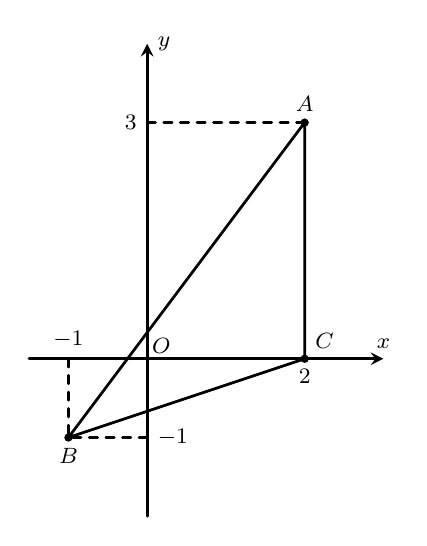
\begin{tikzpicture}[>=stealth,line join=round,line cap=round,line width=1pt,font=\footnotesize]
\draw[->](-1.5,0)--(0,0)node [above right=-2pt]{$ O $}--(3,0) node [above]{$ x $};
\draw[->](0,-2)--(0,4)node [right]{$ y $};
\coordinate[label=above:$A$](A) at (2,3);
\coordinate[label=below:$B$](B) at (-1,-1);
\coordinate[label=above right:$C$](C) at (2,0);
\foreach \toado in {(A),(B),(C)}
{
\fill \toado  circle (1.5 pt);
}
\draw (A)--(B)--(C)--(A);
\draw [dashed] (-1,0)node [above]{$ -1 $}--(B)--(0,-1)node [right]{$ -1 $};
\draw[dashed](0,3)node [left]{$ 3 $}--(A);
\node [below] at (2,0){$ 2 $};
\end{tikzpicture}
\end{center}
Gọi điểm $ C(2 ; 0) $. Suy ra, biểu thức $ T=|z-2|=MC $ (với $ M $ nằm trên đoạn $ AB$).\\
Ta có $ CA=3 $, $ CB=\sqrt{10} $.\\
Suy ra giá trị lớn nhất của biểu thức $ T $ là $ T_{max}=CM_{max}=CB=\sqrt{10}=a $ khi $ M \equiv B $.\\
Biểu thức $T$ đạt giá trị nhỏ nhất là $T_{\min } = CM_{\min }= CH$; với $H$ là hình chiếu vuông góc của điểm $C$ lên đoạn thẳng $AB$.\\
Dễ dàng tìm được đường thẳng $(AB): 4x-3y+1=0$.\\
Suy ra $ CH=d\left(C, AB \right)=\dfrac{9}{5} \Rightarrow T_{min}=CH=\dfrac{9}{5}=b$.\\
Suy ra $ a+b=\sqrt{10}+\dfrac{9}{5} $.
}
\end{ex}

\begin{ex}%[TexBook12-Quyen3-Lam Nguyen]%[2H3K2-3]%
Trong KG $Oxyz$, cho mặt cầu $(S)\colon x^2+y^2+z^2-2x-4y-6z-2=0$ và mặt phẳng $(\alpha)\colon 4x+3y-12z+10=0$. Lập phương trình mặt phẳng $(\beta)$ thỏa mãn đồng thời các điều kiện: tiếp xúc với $(S)$; song song với $(\alpha)$ và cắt trục $Oz$ ở điểm có cao độ dương.
\choice
{$4x+3y-12z-78=0$}
{$4x+3y-12z-26=0$}
{\True $4x+3y-12z+78=0$}
{$4x+3y-12z+26=0$}
\loigiai{
Mặt cầu $(S)$ có tâm $I(1;2;3)$, bán kính $R=\sqrt{1^2+2^2+3^2+2}=4$.\\
Vì $(\alpha)\parallel(\beta)$ nên phương trình $(\alpha)$ có dạng $4x+3y-12z+d=0,\;(d\ne 10 )$.\\
Vì $(\beta)$ tiếp xúc mặt cầu $(S)$ nên $\mathrm{d}(I,(\beta))=R\Leftrightarrow \dfrac{\left| 4\cdot 1+3\cdot  2-12\cdot 3+d \right|}{\sqrt{{4^2+3^2+( -12 )^2}}}=4\Leftrightarrow \left| d-26 \right|=52\Leftrightarrow \hoac{&d=-26 \\& d=78.}$\\
Do $(\beta)$ cắt trục $Oz$ ở điểm có cao độ dương nên chọn $d=78$.\\
Vậy $(\beta)\colon 4x+3y-12z+78=0$.
}
\end{ex}

\begin{ex}%[Thành Đức Trung, Oxyz - Tư duy mở]%[2H3K3-7]%
Trong không gian với hệ trục tọa độ $Oxyz$, cho mặt cầu $\left( S \right)\colon \left( x-1 \right)^2+y^2+\left( z-m \right)^2=25$. Gọi $X$ là tập hợp chứa tất cả các giá trị thực của tham số $m$ để mặt cầu $\left( S \right)$ tiếp xúc với trục $Ox$. Tích tất cả các phần tử của tập hợp $X$ là
\choice
{$25$}
{$-6$}
{\True $-25$}
{$12$}
\loigiai{
Mặt cầu $\left( S \right)\colon \left( x-1 \right)^2+y^2+\left( z-m \right)^2=25$ có tâm $I\left( 1;0;m \right)$ và có bán kính $R=5$.\\
Gọi $H$ là hình chiếu vuông góc của $I\left( 1;0;m \right)$ lên trục $Ox$. Suy ra $H\left( 1;0;0 \right)$.\\
Để mặt cầu $\left( S \right)$ tiếp xúc với trục $Ox$ thì $\mathrm{d}\left( I,Ox \right)=IH=R\Leftrightarrow \left| m \right|=5\Leftrightarrow \hoac{ & m=5 \\ & m=-5.}$\\
Vậy $X=\left\{-5;5 \right\}$. Khi đó tích các phần tử của tập $X$ là $-25$.}
\end{ex}


\Closesolutionfile{ans}